\section{Lagrangian Mechanics}

\epigraph{Nature is thrifty in all its actions.}{Pierre-Louis Moreau de Maupertuis}{wiki: principle of least action ;)}

The term \lingo{generalized coordinates} refers to the parameters that describe the configuration of the system relative to some reference configuration. These parameters must \emph{uniquely} define the configuration of the system relative to the reference configuration. The \lingo{generalized velocities} are the time derivatives of the generalized coordinates of the system.

An example of a generalized coordinate is the angle (anti-clockwise from some reference point) that locates a point moving on a circle. The adjective ``generalized'' distinguishes these parameters from the traditional use of the term coordinate to refer to Cartesian coordinates -- canonical coordinates; \eg, describing the location of the point on the circle using $x$ and $y$ coordinates.

Although there may be many choices for generalized coordinates for a physical system, parameters are usually selected which are convenient for the specification of the configuration of the system and which make the solution of its equations of motion easier. If these parameters are independent of one another, then number of independent generalized coordinates is defined by the number of degrees of freedom of the system.

Finally, canonical coordinates (Cartesian coordinates) all measure lengths, whereas generalized coordinates measure different dimensions; for instance, in polar coordinates $\elset{r, \theta}$, $r$ measures lengths and $\theta$ measures angles; \ie, $\theta$ is dimensionless. Therefore, generalized velocities may not measure in dimensions of length per unit time, generalized momenta may not measure in dimensions of mass times length, generalized forces may not measure in dimensions of mass times length per squared unit time and so on.

\begin{example}
Dynamic model of a simple pendulum. The relationship between the use of generalized coordinates and Cartesian coordinates to characterize the movement of a mechanical system can be illustrated by considering the constrained dynamics of a simple pendulum.
\end{example}

\begin{solution}
A simple pendulum consists of a mass $m$ hanging from a pivot point so that it is constrained to move on a circle of radius $l$. The position of the mass is defined by the coordinate vector $r = \tuple{x\vat t, y\vat t}$ measured in the plane of the circle such that $y$ is in the vertical direction. The coordinates $x\vat t$ and $y\vat t$ are related by the equation of the circle
\beq
f\vat{x\vat t, y\vat t} = x^2\vat t + y^2\vat t - l^2 = x^2 + y^2 - l^2 = 0 \,,
\eeq
that constrains the movement of $m$. This equation also provides a constraint on the velocity components,
\beq
\dt f\vat{x\vat t, y\vat t} 
    = \cder fx \dt x + \cder fy \dt y
    = 2x\vat t x'\vat t + 2y\vat t y'\vat t 
    = 2x \dt x + 2y \dt y \,.
\eeq

Now introduce the parameter $\theta$, that defines the angular position of $m$ from the vertical direction. It can be used to define the coordinates $x\vat t$ and $y\vat t$, such that the coordinate vector
\beq
r = \tuple{x\vat t, y\vat t} = \tuple{l\sin\theta\vat t, -l\cos\theta\vat t} = l\tuple{\sin\theta, \cos\theta}
\eeq
and the velocity becomes
\beq
\dt r = \tuple{l\dt\theta\vat t\cos\theta\vat t, l\dt\theta\vat t\sin\theta\vat t} = l\dt\theta\tuple{\cos\theta, \sin\theta}\,.
\eeq

The use of $\theta\vat t$ to define the configuration of this system avoids the constraint provided by the equation of the circle.
\end{solution}


\subsection{Generalized Coordinates}
A set of \lingo{generalized coordinates} $\elset{\comp q1, \comp q2, \dotsc, \comp qn} = \elset{\comp qi}$ is a set that completely describes the positions of all particles in a mechanical system. In a system with $d\txt f$ degrees of freedom and $k$ constraints, $n = d\txt f - k$ \lingo{independent} generalized coordinates are needed to completely specify all the positions. A \lingo{constraint} is a relation among coordinates, such as $x^2 + y^2 + z^2 = a^2$ for a particle moving on a sphere of radius $a$. In this case, $d\txt f = 3$ and $k = 1$, so we could eliminate $z$ in favor of $x$ and $y$, \ie, by writing $z = \pm\sqrt{a^2 - x^2 - y^2}$, or we could choose as coordinates the polar and azimuthal angles $\theta$ and $\phi$.

For the moment we will assume that $n = d\txt f - k$, and that the generalized coordinates are \emph{independent}, satisfying no additional constraints among them. Later on we will learn how to deal with any remaining constraints among the generalized coordinates $\elset{\comp qi}$.

The generalized coordinates may have dimensions of length, or angle, or perhaps something totally different. In the theory of small oscillations, the normal coordinates are conventionally chosen to have dimensions of $(\phdim{M^{1/2}.L})$. However, once a choice of generalized coordinate is made, with a concomitant set of dimensions, the dimensions of the \lingo{conjugate momentum} $\comp pi$ and \lingo{conjugate force} $\comp fi$ are determined:
\beq
\dim \comp pi = \dfrac{\phdim{M.L^2}}{\phdim T}\dfrac{1}{\dim\comp qi} \qquad \dim \comp fi 
              = \dfrac{\phdim{M.L^2}}{\phdim{T^2}}\dfrac{1}{\dim\comp qi}\,.
\eeq
These choices are such that, if $\comp qi$ has dimensions of length, then $\comp pi$ has dimensions of momentum and $\comp fi$ has dimensions of force. If $\comp qi$ is dimensionless, as is the case for an angle, $\comp pi$ has dimensions of angular momentum ($\phdim{M.L^2/T}$) and $\comp fi$ has dimensions of torque ($\phdim{M.L^2/T^2}$).


\subsection{Principle of Least Action}
In physics, the \lingo{principle of least action} -- or, more accurately, the \lingo{principle of stationary action} -- is a variational principle that, when applied to the action of a mechanical system, can be used to obtain the equations of motion for that system. The principle led to the development of the Lagrangian and Hamiltonian formulations of classical mechanics.

The principle remains \emph{central} in modern physics and mathematics, being applied in the theory of relativity, quantum mechanics and quantum field theory, and a focus of modern mathematical investigation in Morse theory. The chief examples of the principle of stationary action are Maupertuis' principle and Hamilton's principle.

The action principle is preceded by earlier ideas in surveying and optics. The rope stretchers of ancient Egypt stretched corded ropes between two points to measure the path which minimized the distance of separation, and Claudius Ptolemy, in his Geographia (Bk 1, Ch 2), emphasized that one must correct for ``deviations from a straight course''; in ancient Greece Euclid states in his Catoptrica that, for the path of light reflecting from a mirror, the angle of incidence equals the angle of reflection; and Hero of Alexandria later showed that this path was the shortest length and least time. But the credit for the formulation of the principle as it applies to the action is often given to Pierre-Louis Moreau de Maupertuis, who wrote about it in 1744 and 1746. However, scholarship indicates that this claim of priority is not so clear; Leonhard Euler discussed the principle in 1744 and there is evidence that Gottfried Leibniz preceded both by 39 years.

Maupertuis: Credit for the formulation of the principle of least action is commonly given to Pierre-Louis Moreau de Maupertuis, who felt that 
\begin{quote}
Nature is thrifty in all its actions, 
\end{quote}
and applied the principle broadly:
\begin{quote}
The laws of movement and of rest deduced from this principle being precisely the same as those observed in nature, we can admire the application of it to all phenomena. The movement of animals, the vegetative growth of plants [...] are only its consequences; and the spectacle of the universe becomes so much the grander, so much more beautiful, the worthier of its Author, when one knows that a small number of laws, most wisely established, suffice for all movements.
\end{quote}
This notion of Maupertuis, although somewhat deterministic today, \emph{does} capture much of the essence of mechanics.

Lagrange and Hamilton: Much of the calculus of variations was stated by Joseph Louis Lagrange in 1760 and he proceeded to apply this to problems in dynamics. In \lingo{Méchanique Analytique} (1788) Lagrange derived the general equations of motion of a mechanical body. William Rowan Hamilton in 1834 and 1835 applied the variational principle to the classical Lagrangian function
\beq
\lag = \ken - \pen\,,
\eeq
to obtain the \lingo{Euler-Lagrange equations} in their present form.


\subsection{Hamilton's Principle}
The equations of motion of classical mechanics are embodied in a variational principle, called \lingo{Hamilton's principle}. Hamilton's principle states that the motion of a system is such that the \lingo{action functional}
\beq
\action\vat{q\vat t} = \int_{t_1}^{t_2}\, \dx t\, \lag\vat{q, \dt q, t} \,,
\eeq
is an extremum, \ie, $\delta\action = 0$. Here, $q = \elset{\comp qi}$ is a complete set of \lingo{generalized coordinates} for our mechanical system, and
\beq
\lag = \ken - \pen
\eeq
is the \lingo{Lagrangian}, where $\ken$ is the \lingo{kinetic energy} and $\pen$ is the \lingo{potential energy}. Setting the first variation of the action to zero gives the \lingo{Euler-Lagrange equations},
\beq
\eleqn{q}{i} = 0\,,
\eeq
where the first term inside the parenthesis $\cder{\lag}{\comp{\dt q}{i}} = \comp pi$ is the generalized momentum and the second term $\cder{\lag}{\comp{q}{i}} = \comp fi$ is the generalized force. Thus, the Euler-Lagrange equations imply the familiar $\comp{\dt p}{i} = \comp fi$, \aka \lingo{Newton's second law of motion}. Note, however, that the $\elset{\comp qi}$ are generalized coordinates, so $\comp pi$ may not have dimensions of momentum, nor $\comp fi$ of force. For example, if the generalized coordinate in question is an angle $\phi$, then the corresponding generalized momentum is the angular momentum about the axis of $\phi$'s rotation, and the generalized force is the torque.


\subsection{Momentum conservation}
Whenever $\lag$ is independent of a generalized coordinate $\comp qi$, the conjugate force $\comp fi$ vanishes and therefore the conjugate momentum $\comp pi$ is conserved. This is an example of a deep result known as \lingo{Noether's theorem}. Noether's theorem guarantees that to every \emph{continuous symmetry of $\lag$} there corresponds an associated \lingo{conserved quantity}.


\subsection{Invariance of the equations of motion}
The equations of motion are \emph{invariant under a shift of $\lag$} by a total time derivative of a function of coordinates and time.


\subsection{Remarks on the Choice of Generalized Coordinates}
Any choice of generalized coordinates will yield an equivalent set of equations of motion. However, some choices result in an apparently simpler set than others. This is often true with respect to the form of the potential energy. Additionally, certain constraints that may be present are more amenable to treatment using a particular set of generalized coordinates.

The kinetic energy $\ken$ is always simple to write in Cartesian coordinates, and it is good practice, at least when one is first learning the method, to write $\ken$ in Cartesian coordinates and then convert to generalized coordinates. In Cartesian coordinates, the kinetic energy of a single particle of mass $m$ is
\beq
\ken = \tfrac{1}{2}m(\dt x^2 + \dt y^2 + \dt z^2)\,.
\eeq

If the motion is two-dimensional, and confined to the plane $z = \text{const.}$, one $2\ken = m(\dt x^2 + \dt y^2)$.

Two other commonly used coordinate systems are the cylindrical and spherical systems. In cylindrical coordinates $\tuple{\rho, \phi, z}$, $\rho$ is the radial coordinate in the $\tuple{x,y}$ plane and $\phi$ is the azimuthal angle:
\begin{align*}
& x = \rho\cos\phi    & \dt x = \dt\rho\cos\phi - \rho\dt\phi\sin\phi \,,\\
& y = \rho\sin\phi    & \dt y = \dt\rho\sin\phi + \rho\dt\phi\cos\phi \,.
\end{align*}
and the third, orthogonal coordinate is $z$. The kinetic energy is then
\beq
\ken = \tfrac{1}{2}m(\dt x^2 + \dt y^2 + \dt z^2) = \tfrac{1}{2}m(\dt\rho^2 + \rho^2\dt\phi^2 + \dt z^2) \,.
\eeq
When the motion is confined to a plane with $z = \text{const.}$, this coordinate system is often referred to as ``two-dimensional polar'' coordinates.


\subsection{How to Solve Mechanics Problems}
Here are some simple steps you can follow toward obtaining the equations of motion:
\begin{enumerate}
\item Choose a set of generalized coordinates $\elset{\comp q1, \dotsc, \comp qn}$.
%
\item Find the kinetic energy $\ken\vat{q, \dt q, t}$, the potential energy $\pen\vat{q,t}$ and the Lagrangian $\lag\vat{q,\dt q, t} = \ken - \pen$. It is often helpful to first write the kinetic energy in Cartesian coordinates for each particle before converting to generalized coordinates.
%
\item Find the canonical momenta $\comp pi = \cder{\lag}{\comp{\dt q}{i}}$ and the generalized forces $\comp fi = \cder{\lag}{\comp qi}$.
%
\item Evaluate the time derivatives $\comp{\dt q}{i}$ and write the equations of motion $\comp{\dt p}{i} = \comp fi$. Be careful to differentiate properly, using the chain rule and the Leibniz rule where appropriate.
%
\item Identify any conserved quantities.
%
%
\item Note about wording: when using Cartesian coordinates, \aka, canonical coordinates, all of the quantities are named \lingo{canonical}; \eg, canonical coordinates, canonical momentum, canonical force and so on. When using other coordinates, \aka, generalized coordinates, all of the quantities are named \lingo{generalized}; \eg, generalized coordinates, generalized momentum, generalized force and so on. 
%
\item Note about physical interpretation: the generalized quantities have physical interpretations depending on the underling coordinates being used.
\end{enumerate}


\subsection{Examples}
Find the equation of one-dimensional motion. 

\begin{solution}
Use Cartesian coordinates -- canonical coordinates. Then, choose the canonical coordinate $x$ to describe the one-dimensional mechanical system. These system has potential energy $\pen\vat x$ and, thus, the Lagrangian is
\beq
\lag = \ken - \pen = \tfrac{1}{2}m \dt x^2 - \pen\vat x\,.
\eeq

The canonical momentum (canonical because we are using Cartesian coordinates) is 
\beq
p = \xpd{\lag}{\comp{\dt x}{}} = m\dt x\,.
\eeq
and the canonical force
\beq
f = \xpd{\lag}{\comp{x}{}} = \pen'\vat x\,.
\eeq

The equation of motion is finally
\beq
\eleqn{x}{} = 0 \implies m\ddt x = -\pen'\vat x\,,
\eeq
which is $f = ma$.

Note that we can multiply the equation of motion by $\dt x$ to get
\beq
0 = m\dt x\left(m\ddt x + \pen'\vat x \right) 
  = \xod{}{t}\Bigl(\tfrac{1}{2}m\dt x^2 + \pen\vat x \Bigr) 
  = \xod{E}{t} 
  = \dt E\,,
\eeq
where $E = \ken + \pen$ is the total energy of the system.
\end{solution}


\begin{example}
Consider next a particle of mass $m$ moving in two dimensions under the influence of a potential $\pen\vat\rho$ which is a function of the distance from the origin $\rho^2 = x^2 + y^2$. Find the equations of motion.
\end{example}

\begin{solution}
Using polar coordinates, the Lagrangian becomes
\beq
\lag = \tfrac{1}{2}m\left(\dt\rho^2 + \rho\dt\phi^2\right) + \pen'\vat\rho\,.
\eeq

The equations of motions via the Euler-Lagrange equations are
\begin{align*}
& \eleqn{\rho}{} = m\ddt\rho - m\rho\dt\phi^2 + \pen'\vat\rho \,,\\
& \eleqn{\phi}{} = 0 \implies \xod{}{t}\left(m\rho^2\dt\phi\right) = 0\,.
\end{align*}

Note that the canonical momentum conjugate to $\phi$, which is to say the angular momentum, is conserved
\beq
\comp p\phi = m\rho^2\dt\phi = \text{const.}\,.
\eeq
Use this to eliminate $\dt\phi$ from the first Euler-Lagrange equation to obtain
\beq
m\ddt\rho = \dfrac{(\comp p\phi)^2}{m\rho^3} - \pen'\vat\rho\,.
\eeq

The total energy $E = \ken + \pen$ can then be written as
\beq
E = \tfrac{1}{2}m\dt\rho^2 + \dfrac{(\comp p\phi)^2}{m\rho^3} + \pen\vat\rho\,,
\eeq
from which it may be shown that $E$ is also a constant:
\beq
\xod Et = \left( m\ddt\rho - \dfrac{(\comp p\phi)^2}{m\rho^3} + \pen'\vat\rho \right)\dt\rho = 0 \,.\mqed
\eeq
\end{solution}


\subsection{Conserved Quantities}
A conserved quantity $\Lambda\vat{q,\dt q,t}$ is one which does not vary throughout the motion of the system. This means
\beq
\xod\Lambda t\biggl\vert_{q = q\vat t} = 0\,.
\eeq

Momentum conservation: The simplest case of a conserved quantity occurs when the Lagrangian does \emph{not} explicitly depend on one or more of the generalized coordinates, \ie, when
\beq
\comp fi = \xpd \lag{\comp qi} = 0\,.
\eeq
We then say that $\lag$ is \lingo{cyclic in the coordinate $\comp qi$} (\ie, when the generalized force in the coordinate $\comp qi$ vanishes). In this case, the Euler-Lagrange equations $\comp{\dt p}{i} = \comp fi$ say that the conjugate momentum $\comp pi$ is conserved. (This case is the exact analog to the Newtonian formalism: when there are no forces acting on a particle, the particle linear momentum is preserved: $\dt p = f$, but $f = 0$. Thus, $\dt p = 0$, or $p$ is constant.)


\begin{example}
Consider the motion of a particle of mass $m$ near the surface of the earth. Let $\tuple{x,y}$ be coordinates parallel to the surface and $z$ the height. Find the equations of motion.
\end{example}

\begin{solution}
The Lagrangian for the particle motion is
\beq
\lag = \ken - \pen = \tfrac{1}{2}m\left(\dt x^2 + \dt y^2 + \dt z^2\right) - mgz\,.
\eeq

Since $\comp fx = \cder\lag x = 0$ and $\comp fy = \cder\lag y = 0$, then $\comp px$ and $\comp py$ are conserved with
\beq
\comp px = \xpd\lag{\dt x} = m\dt x\qquad\text{and}\qquad
\comp py = \xpd\lag{\dt y} = m\dt y\,.
\eeq

Integrate the first order Euler-Lagrange equations to yield
\beq
x\vat t = x\vat 0 + \tfrac{\comp px}{m}t\qquad\text{and}\qquad
y\vat t = y\vat 0 + \tfrac{\comp py}{m}t\,.
\eeq

The $z$ equation is
\beq
\comp{\dt p}{z} = m\ddt z = -mg = \comp fz\,,
\eeq
with solution
\beq
z\vat t = z\vat 0 + \dt z\vat 0 t - \tfrac{1}{2}g t^2\,.\mqed
\eeq
\end{solution}


\subsection{Summary of Lagrangian mechanics}

[advanced mechanics, Eric Poisson]

The methods of Newtonian mechanics, based on the vectorial equation $f = \dt q$, are very powerful and they can be applied to \emph{all} mechanical systems. But they lack in efficiency when Cartesian coordinates $\tuple{x,y,z}$ do not give the simplest description of a mechanical system.

To increase the efficiency of the theoretical methods of mechanics, a number of scientists in the centuries following Newton endeavored to recast the Newtonian laws into a more flexible formulation. The most famous players include Leonhard Euler (1707-1783), Joseph Lagrange (1736-1813), William Rowan Hamilton (1805-1865), and Carl Gustav Jacobi (1804-1851). Their new techniques proved extremely useful and they allowed them and others to solve increasingly challenging problems, most notably in the context of celestial mechanics. These new powerful techniques are the topic of this chapter on Lagrangian mechanics and the following chapter on Hamiltonian mechanics.

It is important to point out that 
\begin{quote}
the Lagrangian and Hamiltonian formulations of the laws of mechanics are largely restricted to forces that can be derived from a potential; \ie, conservative forces.
\end{quote}
For other problems, such as a particle subjected to air resistance, the new techniques cannot be applied in a very straightforward way and it is usually best to go back to the old Newtonian methods. In this chapter and the next, we shall consider only forces that can be derived from a potential.

The entire content of Lagrangian mechanics is summarized in the following simple recipe:
\begin{enumerate}
\item Verify the applicability of the Lagrangian formalism: forces must be conservative, for only then they can be expressed as a potential: $f\txt{cons} = -\gder\pen$. (Conservative forces depend only on the position vector $f\txt{cons}\vat{x,t}$, whereas non-conservative forces on position and velocity $f\txt{non-cons}\vat{x, \dt x,t}$.)
%
\item Select generalized coordinates $\setprop{\comp qi}{i = 1,2,\dotsc}$ to describe the degrees of freedom of a mechanical system. These coordinates are completely \emph{arbitrary}. They need not be the original Cartesian coordinates associated with an inertial frame. Indeed, there is no need for the coordinates to even be attached to an inertial frame. The index $i$ labels each one of the generalized coordinates; there is one coordinate for each degree of freedom.
%
\item In terms of the generalized coordinates, calculate the system's total kinetic energy $\ken$ and total potential energy $\pen$. Then form what is known as the Lagrangian function of the system, denoted $\lag\vat{\comp qi, \comp{\dt q}{i}}$; this depends on the generalized coordinates $\comp qi$ and the generalized velocities $\comp{\dt q}{i} \defby \dx q/\dx t$. The Lagrangian is defined by $\lag = \ken - \pen$; it is the \emph{difference} between the kinetic and potential energies.
%
\item Substitute the Lagrangian into the Euler-Lagrange (EL) equations,
\beq
\eleqn{q}{i} = 0\,.
\eeq
This returns \emph{an equation of motion for each generalized coordinate $\comp qi\vat t$}; \ie, there is one EL equation for each generalized coordinate.
%
\item Identify any conserved quantities.
%
\item The rest of the recipe is concerned with solving the equations of motion. The methods for doing this are varied, and they depend on the particular situation, just as they do in the Newtonian formulation.
%
\item Note about wording: when using Cartesian coordinates, \aka, canonical coordinates, all of the quantities are named \lingo{canonical}; \eg, canonical coordinates, canonical momentum, canonical force and so on. When using other coordinates, \aka, generalized coordinates, all of the quantities are named \lingo{generalized}; \eg, generalized coordinates, generalized momentum, generalized force and so on. 
%
\item Note about physical interpretation: the generalized quantities have physical interpretations depending on the underling coordinates being used.
\end{enumerate}

Let us first verify that the recipe is compatible with Newton's laws. 

\begin{example}
Consider a particle moving in three-dimensional space and subjected to a potential $\pen\vat{x,y,z}$. Describe the motion of the particle using Cartesian coordinates -- canonical coordinates.
\end{example}

\begin{solution}
In this case, therefore, the generalized coordinates are chosen as $\comp q1 = x$, $\comp q2 = y$ and $\comp q3 = z$. The particle's kinetic energy is $2\ken = m(\dt x^2 + \dt y^2 + \dt z^2)$ and the Lagrangian function is
\beq
\lag\vat{x,y,z,\dt x,\dt y,\dt z} = \tfrac{1}{2}m(\dt x^2 + \dt y^2 + \dt z^2) - \pen\vat{x,y,z}\,.
\eeq
To substitute this into the EL equation for $\comp q1 = x$, say, we must first evaluate the generalized momentum $\comp px = \cder L{\dt x}$. This is the partial derivative of $\lag$ with respect to $\dt x$, treating all other variables (including $x$) as constant parameters. This is given by
\beq
\comp px = \xpd{\lag}{\dt x} = m\dt x\,.
\eeq
(The generalized momentum coincides with the canonical momentum, since we're using Cartesian coordinates.)

We next differentiate this with respect to $t$ to get the rate change of generalized momentum $\comp{\dt p}{x}$:
\beq
\comp{\dt p}{x} = \xod{}{t}\xpd{\lag}{\dt x} = m\ddt x\,.
\eeq

Finally, we partially differentiate $\lag$ with respect to $x$, treating all other variables (including $\dt x$) as constant parameters; this gives the generalized force $\comp fx$:
\beq
\comp fx = \xpd\lag x = -\xpd\pen x\,.
\eeq
(The generalized force coincides with the canonical force, since we're using Cartesian coordinates.)

Substituting these results into the EL equation for $x$, we arrive at
\beq
\eleqn x{} = 0\implies m\ddt x + \xpd\pen x = 0 \,.
\eeq

Repeating these calculations for $y$ and $z$ would eventually return the full vectorial equation
\beq
ma + \gder\pen = 0\,.
\eeq
or $ma = f$ if we recall that the force is derived from the potential, so that $f = -\gder\pen$. This exercise reveals that indeed, 
\begin{quote}
the Lagrangian recipe is compatible with the Newtonian law.
\end{quote}
\end{solution}


The true power of the recipe, however, is revealed when the generalized coordinates are not Cartesian, not canonical. Let us see what the recipe produces in the case of a pendulum. 

\begin{example}
Find the equations of motion for a pendulum.
\end{example}

\begin{solution}
The pendulum's single degree of freedom is best represented by the swing angle $\theta$; this will be our generalized coordinate for this problem and we write $q = \theta$. (We do not need a label, index, $i$ in this case, as there is only one generalized coordinate.) The relation between $\theta$ and the original Cartesian coordinates is $x = l\sin\theta$ and $z = l\cos\theta$, with $l$ denoting the length of the rod. The pendulum's kinetic energy is $2\ken = m(\dt x^2 + \dt z^2)$. Its potential energy is $\pen = -mgz = -mgl\cos\theta = -ml^2\omega^2\cos\theta$, where we have introduced the quantity $\omega^2 = g/l$. The pendulum's Lagrangian function is
\beq
\lag\vat{\theta,\dt\theta} = ml^2\left(\tfrac{1}{2}\dt\theta^2 + \omega^2\cos\theta\right)\,.
\eeq

To substitute this into the EL equation we must first evaluate the generalized momentum $\comp p\theta$ -- the partial derivative of $\lag$ with respect to $\dt\theta$. This is
\beq
\comp p\theta = \xpd{\lag}{\dt \theta} = ml^2\dt\theta\,.
\eeq

Next we calculate the change in momentum $\comp{\dt p}{\theta}$ -- we differentiate the last equation with respect to time:
\beq
\comp{\dt p}{\theta} = \xod{}{t}\xpd{\lag}{\dt \theta} = ml^2\ddt\theta \,.
\eeq

Finally, we calculate the generalized force $\comp f\theta$ -- the partial derivative of $\lag$ with respect to $\theta$:
\beq
\comp f\theta = \xpd{\lag}{\theta} = ml^2\ddt\theta\,.
\eeq

Substituting these results into the EL equation produces:
\beq
\comp{\dt p}{\theta} - \comp{f}{\theta} = 0 
    \implies ml^2\left(\ddt\theta + \omega^2\sin\theta\right) = 0 
    \implies \ddt\theta + \omega^2\sin\theta = 0\,.
\eeq
This last equation can also be obtained by Newtonian methods -- the calculation is fairly laborious. However, comparing the computations carried out here to those required by Newtonian methods shows the greater efficiency of the Lagrangian recipe.
\end{solution}


\subsection{The Classical Lagrangian}

[advanced mechanics and general relativity, joel franklin]

\subsubsection{The Lagrangian}
A Lagrangian is the integrand of an action -- while this is not the usual definition, it is, upon definition of action, more broadly applicable than the usual ``kinetic minus potential'' form. In classical mechanics, the Lagrangian leading to Newton's second law reads, in Cartesian coordinates, with $r\vat t$ being the position vector:
\beq
\lag \defby \tfrac{1}{2}m\,\dt r\vat t\iprod \dt r\vat t - \pen\vat{r\vat t}
      = \tfrac{1}{2}m\,v\vat t\iprod v\vat t - \pen\vat{r\vat t}\,,
\eeq
where we view $x$, $y$ and $z$ as functions of a parameter $t$ which we normally interpret as ``time''. The first term is the kinetic energy (denoted $\ken$), the second is the potential energy. Remember, the ultimate goal of classical mechanics is to find the trajectory of a particle under the influence of a force. Physically, we control the description of the system by specifying the particle mass, form of the force or potential and boundary conditions (particle starts from rest, particle moves from point $\point A$ to point $\point B$, \etc.). Mathematically, we use the equations of motion derived from the Lagrangian, together with the boundary conditions, to determine the curve $r\vat t = \comp{x}{k}\vat t\ifvec k$ through three-dimensional space with a frame $\frm k$.

Calculus of Variations provides the ordinary differential equation (ODE) structure of interest, a set of three second-order differential equations, the Euler-Lagrange equations of motion:
\begin{equation}\label{eq:eulerlageqnsvectorform}
\xod{}{t}\xpd\lag v - \xpd\lag r = 0 \implies \xod{}{t}\xpd\lag{\dt r} - \xpd\lag r = 0\,,
\end{equation}
where we identify the particle's momentum $p = \cder\lag v$ and force on the particle $f = \cder\lag r = -\gder\pen$ (note that since $f = -\gder\pen$, the force must be conservative; \ie, only a function of position and not velocity). With these identifications, the Euler-Lagrange equations could be written as $\dt p = f$, which is precisely Newton's second law of motion.

The advantage of the action approach, and the Lagrangian in particular, is that the equations of motion can be obtained for \emph{any} coordinate representation of the kinetic energy and potential. Although it is easy to define and verify the correctness of the Euler-Lagrange equations in Cartesian coordinates, they are \emph{not necessary} to the formulation of valid equations of motion for systems in which Cartesian coordinates are less physically and mathematically useful.

The Euler-Lagrange equations, in the form \cref{eq:eulerlageqnsvectorform}, hold regardless of our association of $r$, the position vector, with Cartesian coordinates. Suppose we move to cylindrical coordinates $\tuple{\rho,\phi,z}$, defined by
\beq
x = \rho\cos\phi\,,\qquad y = \rho\sin\phi\qquad\text{and}\qquad z = z\,,
\eeq
then the Lagrangian in Cartesian coordinates can be transformed to cylindrical coordinates by making the replacement for $\tuple{x,y,z}$ in terms of $\tuple{\rho,\phi,z}$ (and associated substitutions for the Cartesian velocities):
\beq
\lag\vat{\rho,\phi, z} = \lag\vat{r\vat{\rho,\phi, z}} 
                   = \tfrac{1}{2}m\left(\dt \rho^2 + \dt\phi^2 + \dt z^2\right) - \pen\vat{\rho,\phi,z}\,.
\eeq

But, the Euler-Lagrange equations require no modification, the variational procedure that gave us \cref{eq:eulerlageqnsvectorform} can be applied in the cylindrical coordinates, giving three equations of motion:
\beq
\begin{cases}
\eleqn{\rho}{}    = 0\,,\\
\eleqn{\phi}{} = 0\,,\\
\eleqn{z}{}    = 0\,.
\end{cases}
\eeq

The advantage is clear: \emph{coordinate transformation occurs once and only once, in the Lagrangian}. If we were to start with Newton's second law, we would have three equations with acceleration and coordinates coupled together. The decoupling of these would, in the end, return into the last set of equations.


\subsubsection{Metric Tensor}
In the mathematical field of differential geometry, a \lingo{metric tensor} is a type of function defined on a manifold (such as a surface in space) which takes as input a pair of tangent vectors $v$ and $w$ and produces a real number (scalar) $\metric\vat{v,w}$ in a way that generalizes many of the familiar properties of the dot product of vectors in Euclidean space. In the same way as a dot product, metric tensors are used to define the length of, and angle between, \emph{tangent vectors}.

[axioms of metric tensor: \url{https://en.wikipedia.org/wiki/Metric_tensor#Definition}]

Basically, a generic metric should be bilinear, symmetric and nondegenarated.

Consider a region $\nset Vn$ in $\nset Rn$. Then, define the \lingo{metric tensor}, denoted $\metric$, by
\beq
\metric\vat{x,y} \defby \sstep{xy} = x\iprod y\,.
\eeq

Agree on calling the metric tensor simply \lingo{metric}.

\begin{remark}
The metric tensor is \emph{not} the same as the Euclidean metric. The Euclidean metric requires that if a vector is inserted in its two slots, the output should be zero! On the contrary, the metric tensor produces the length of a vector in such a case. Thus, the metric tensor behaves more like the Euclidean norm or magnitude, in GA.

Odd the name!
\end{remark}


\subsubsection{Geometric Form of the Lagrangian}
Consider three points $\point P, \point Q, \point O\in\espace 3$. Relative to $\point O$, denote the position of $\point P$ by the vector $\pvec\vat{\point P}$ and the position of $\point Q$ by the vector $\pvec\vat{\point Q}$. Then, define the \lingo{separation between two points}, denoted $\svec$, by
\beq
\diff\svec \defby \pvec\vat{\point P} - \pvec\vat{\point Q} = \diff\pvec_{\point P, \point Q}\,.
\eeq

Assume $\point P$ and $\point Q$ were so close to each other, so to write $\dx\svec = \dx\pvec$. Refer to $\dx\svec$ as the \lingo{differential separation vector}.

Define, then, the \lingo{squared differential length}, denoted $\dx\svec^2$, by
\beq
\dx\svec^2 \defby \dx\pvec^2 = \dx\pvec\,\dx\pvec = \dx\pvec\iprod\dx\pvec\,,
\eeq
since $\dx\pvec$ is colinear to itself; \ie, $\dx\pvec\oprod\dx\pvec = 0$. Note that, by the contraction axiom, $\dx\svec^2$ is a scalar.

In terms of the metric, the squared differential length becomes
\beq
\dx\svec^2 = \metric\vat{\dx\pvec, \dx\pvec}\,.
\eeq

Now, consider a particle of mass $m$ moving under the interaction~\footnote{~Since the interaction comes from a potential, the force on the particle must be conservative; \ie, it should depend exclusively on the particle position $f\vat\pvec$. Only then does one have $f = -\gder\pen$.} with a \lingo{potential} $\pen\vat\pvec$. Then, define the \lingo{particle kinetic energy}, denoted $\ken$, by
\beq
\ken\vat{\dt\pvec} \defby \tfrac{1}{2}m\,v^2 
                    = \dfrac{1}{2}m\,v\iprod v 
                    = \dfrac{1}{2}m\,\dt\pvec\iprod\dt\pvec 
                    = \dfrac{1}{2}m\,\metric\vat{\dt\pvec,\dt\pvec}\,.
\eeq

With this result, define the \lingo{particle Lagrangian}, denoted $\lag$, by
\beq
\lag\vat{\pvec, \dt\pvec} = \ken - \pen 
                          = \tfrac{1}{2}m\,\dt\pvec\iprod\dt\pvec - \pen\vat\pvec 
                          = \tfrac{1}{2}m\,\metric{\dt\pvec,\dt\pvec} - \pen\vat\pvec \,.
\eeq

With the last equation, find the Euler-Lagrange equations, which lead to the equations of motion:
\beq
\eleqn{x}{} = 0\,.
\eeq

\begin{remark}
In the above equation, $\pvec$ and $\dt\pvec$ represent the particles' position and velocity, both of them are \emph{vectors}.
\end{remark}

Refer to the term $\cder{\lag}{\dt\pvec}$ as \lingo{momentum} and to the term $\cder{\lag}{\pvec}$ \lingo{force}. See that the force comes from the potential; \ie, $\cder{\lag}{\pvec} = -\gder\pen\vat\pvec$.

Finally, note the use of the \lingo{geometric principle} applied to physics throughout this section: \emph{no} coordinate systems -- thus \emph{no} components, coordinates neither unit vectors -- were required to define points, separation vector, distance, metric, mass, potential and kinetic energy and Lagrangian, since they are all geometric objects.


\subsubsection{Equations of Motion in Index Notation}
Consider now a coordinate system with a basis $\set B$ for $\espace 3$. Then, express vectors by its components onto the basis, say $a = \comp ai$, where the indices $i,j$ run from 1 to 3. Then, the length of a vector is given by the metric (tensor)
\beq
\metric\vat{a,a} = \imet ij\comp ai\comp aj\,,
\eeq
where the numbers $\elset{\imet ij}$ are called the \lingo{metric elements onto the basis $\set B$}.

By letting $\pvec$ to represent the position vector, by noting that velocity is defined as $v = \dt\pvec$ and by using the metric elements, express thus the Lagrangian of a particle of mass $m$ moving under a potential $\pen\vat x$ as
\beq
\lag = \tfrac{1}{2} m\,\imet ij\comp{\dt x}{i}\,\comp{\dt x}{j} - \pen\vat x\,.
\eeq
Refer to the last equation as the \lingo{index form of the Lagrangian}.

\begin{remark}
The index form of the Lagrangian does \emph{not} directly express any particular coordinate system -- it works for them all.
\end{remark}

Finally, the Euler-Lagrange equations, which lead to the equations of motion, are in index notation
\beq
\eleqn{x}{i} = 0\,.
\eeq

\begin{caution}
Be careful! It is possible (as in the spherical case) that the metric depends on the coordinates; \ie, $\metric\vat{\pvec}$. So, use the chain rule and the Leibniz rule where appropriate when deriving the equations of motion from the Euler-Lagrange equations.
\end{caution}


\subsection{Lagrangian Coordinate Transformation Recipe}
It is possible to go from canonical coordinates (cartesians) directly to other coordinate systems and find the form of the Lagrangian without directly transforming it, but, indirectly, using the metric.

\begin{example}
Transform the Lagrangian from Cartesian coordinates to spherical coordinates using the metric.
\end{example}

\begin{solution}
First, write the differential distance in both coordinate systems:
\beq
\begin{cases}
\dx\svec^2 = \dx x^2 + \dx y^2 + \dx z^2\,,                                 &\eqtxt{Cartesian coordinates}\\
\dx\svec^2 = \dx r^2 + r^2\,\dx\theta^2 + r^2\,\sin^2\theta\,\dx\theta^2\,. &\eqtxt{spherical coordinates}
\end{cases}
\eeq

Rewrite the differential distance in matrix notation using cartesians
\beq
\dx\svec^2 = \begin{bmatrix} \dx x & \dx y & \dx z \end{bmatrix}
             \begin{bmatrix}
                 1 & 0 & 0 \\
                 0 & 1 & 0 \\
                 0 & 0 & 1
             \end{bmatrix}
             \begin{bmatrix} \dx x \\ \dx y \\ \dx z \end{bmatrix}\,.
\eeq

Rewrite the differential distance in matrix notation using sphericals
\beq
\dx\svec^2 = \begin{bmatrix} \dx r & \dx \theta & \dx \phi \end{bmatrix}
             \begin{bmatrix}
                 1 & 0   & 0 \\
                 0 & r^2 & 0 \\
                 0 & 0   & r^2\sin^2\theta
             \end{bmatrix}
             \begin{bmatrix} \dx r \\ \dx \theta \\ \dx \phi \end{bmatrix}\,.
\eeq

Next, write the Lagrangian in matrix notation using cartesians
\beq
\lag = \tfrac{1}{2}m \begin{bmatrix} \dt x & \dt y & \dt z \end{bmatrix}
                     \begin{bmatrix}
                         1 & 0 & 0 \\
                         0 & 1 & 0 \\
                         0 & 0 & 1
                     \end{bmatrix}
                     \begin{bmatrix} \dt x \\ \dt y \\ \dt z \end{bmatrix}
        - \pen\vat{x,y,z}\,.
\eeq

Finally, write the Lagrangian in matrix notation using sphericals
\beq
\lag = \tfrac{1}{2}m \begin{bmatrix} \dt r & \dt \theta & \dt \phi \end{bmatrix}
                     \begin{bmatrix}
                         1 & 0   & 0 \\
                         0 & r^2 & 0 \\
                         0 & 0   & r^2\sin^2\theta
                     \end{bmatrix}
                     \begin{bmatrix} \dt r \\ \dt \theta \\ \dt \phi \end{bmatrix}
        - \pen\vat{x,y,z}\,.\mqed
\eeq
\end{solution}

Noting the similarities between the equations in the last example, write a prescription to transform the Lagrangian to \emph{any} coordinate system:
\begin{enumerate}
\item Define the coordinate system to work in and express its relationship to Cartesian coordinates. Calculate the differential separation between points and then the squared differential length in such a system. Note the metric elements of the squared differential length. (This is due to the relationship between the metric and the differential length: they are the same! Both measure distances, but have different form. So, if we know the squared differential length, we know the metric elements and, the other way around, if we know the metric elements, we can find the differential distance.)
%
\item Write the kinetic energy in Cartesian coordinates and there replace the metric coefficients and replace the coordinate differentials with the coordinate distances; \eg, in Cartesians, the coordinate differentials are $\tuple{\dx x, \dx y, \dx z}$ and the coordinate distances are $\tuple{\dt x, \dt y, \dt z}$. This means transform the $\dx x$'s into $\dt x$'s.
%
\item Finally, express the Lagrangian in the chosen coordinate system.
\end{enumerate}

The trick works from the realization that the differential distance and the kinetic energy (the part of the Lagrangian we want to transform) have similar \emph{structure}. In index notation:
\begin{align*}
\dx\svec^2 &\sim \dx x\iprod \dx x \sim\metric\vat{\dx x, \dx x} \sim \imet ij\,\comp{\dx x}{i}\comp{\dx x}{j}\,,\\
         k &\propto v\iprod v \propto \dt x\iprod\dt x \propto \metric\vat{\dt x, \dt x} 
            \propto \imet ij\,\comp{\dt x}{i}\comp{\dt x}{j}\,.
\end{align*}
Besides the $m/2$ factor omitted in the kinetic energy, the only difference between the two equations is that the $\dx x$'s in the differential distance changed into $\dt x$'s in the kinetic energy. The metric coefficients are, however, the same!

Remember, finally, that the differential distance, the metric, the kinetic energy and the Lagrangian are geometric objects, they need not coordinate systems for their definitions. Nevertheless, for expressing results and calculations, different \emph{representations} of these objects in different coordinate systems are required. The metric is the object that enables such transformations between geometric objects from one representation to another.


\subsection{Lagrangian Coordinate Transformation Recipe -- Revisited}
Relationship among the particle position $\pvec$, the particle kinetic energy $\ken$ and the metric $\metric$ in any coordinate system:

Consider an $n$-dimensional Euclidean space $\espace n$. Consider a frame for $\espace n$ with elements $\frm k$; the frame need not be normal nor orthogonal. Then, project $\pvec$ onto the frame -- write $\pvec$ as linear combination of the frame elements:
\beq
\pvec = \ifvec k\comp\pvec k\,.
\eeq

Find $\dx\pvec$ and then $\dx^2\pvec = \dx\pvec\dx\pvec = \dx\pvec\iprod\dx\pvec$
\beq
  \dx\pvec = \ifvec k\dx\comp\pvec k\implies
\dx^2\pvec = \imet kl\comp\pvec k\comp\pvec l\,,
\eeq
since $\ifvec k\iprod\ifvec l = \imet kl$.

Calculate the particle velocity $\dt\pvec$ and square it; \ie, $\dt\pvec\dt\pvec$:
\beq
\dt\pvec = \xod{\pvec}{t}\implies
\dt\pvec\dt\pvec = \imet kl\cntens{\dt\pvec} k\cntens{\dt\pvec} l
\eeq
and calculate then the particle kinetic energy $\ken$
\beq
\ken = \dfrac{1}{2}m\dt\pvec\dt\pvec
     = \dfrac{1}{2}m\imet kl\cntens{\dt\pvec} k\cntens{\dt\pvec} l\,.
\eeq

Notice, finally, that during the calculation the metric coefficients have not changed when going from $\dx^2\pvec$ to $\ken$! That's why the trick of using the line element to find $\imet kl$ and using them directly to calculate the kinetic energy works.



\subsection{Lagrangian in Various Coordinate Systems}
While geometric objects have the same form independently on the coordinate system in use, their \emph{representations} onto coordinate systems (\ie, components or coordinates) vary from one system to another. However, sometimes working with one particular coordinate system makes calculations and understanding and calculations easier than with others. Therefore, knowing how to move from one system to another is imperative. This is the topic of this section.


\subsubsection{Lagrangian in Cartesian Coordinate Systems}
In Cartesian coordinates, find the position of a particle by means of the set $\elset{x,y,z}$, where all of the set elements measure lengths from the particle to the coordinate axes. Use as a basis for the coordinate system the~\footnote{~The set $\elset{\nvec x, \nvec y, \nvec z}$ is traditionally written as $\elset{\hat\imath, \hat\jmath, \hat k}$.} set $\elset{\nvec x, \nvec y, \nvec z}$, where the set elements are normal and orthonormal to each other; \ie, the chosen basis is orthonormal. The position vector is thus $\pvec = x\,\nvec x + y\,\nvec y + z\,\nvec z$; whereas the differential separation is $\dx\svec = \dx x\,\nvec x + \dx y\,\nvec y + \dx z\,\nvec z$. Next, the differential distance is given by
\beq
\dx\svec^2 = \dx x^2 + \dx y^2 + \dx z^2\,.
\eeq

Next, the metric elements are given in matrix representation by~\footnote{~Since Cartesian coordinates directly measure lengths, then expect no change in the metric coefficients.} $\mtrx\metric = \imet ij = \diag\tuple{1,1,1}$, where $i$ represent the matrix rows and $j$ columns.

\begin{note}
By definition of the metric in index notation, read the metric coefficients directly from the differential distance. On the contrary, if the metric coefficients are given, then the differential distance can be directly formed from the metric coefficients.
\end{note}

Finally, the Lagrangian is given by
\beq
\lag = \tfrac{1}{2} m\,\imet ij\comp{\dt x}{i}\,\comp{\dt x}{j} - \pen\vat{x,y,z} 
     = \tfrac{1}{2} m (\dt x^2 + \dt y^2 + \dt z^2) - \pen\vat{x,y,z} \,.
\eeq

\begin{note}
To find the form of the particle kinetic energy, take the differential distance terms and replace the $\elset{\dx x^2}$'s by $\elset{\dt x^2}$'s, leaving the coefficients of the metric untouched.
\end{note}


\subsubsection{Lagrangian in Cylindrical Coordinate Systems}
In cylindrical coordinates, find the position of a particle by means of the set $\elset{\rho,\phi,z}$. Transform between Cartesians and cylindricals by
\beq
x = \rho\cos\phi\,,\qquad y = \rho\sin\phi\qquad\text{and}\qquad z = z\,.
\eeq
Here, $\rho$ and $z$ measure lengths while $\phi$ angles, so expect the metric coefficients to be different from unity.

Use as a basis for the system the set $\elset{\nvec\rho, \nvec\phi, \nvec z}$. The differential separation is then $\dx\svec = \dx\rho\,\nvec\rho + \rho\,\dx\phi\,\nvec\phi + \dx z\,\nvec z$. The differential distance thus is
\beq
\dx\svec^2 = \dx\rho^2 + \rho^2\,\dx\phi^2 + \dx z^2\,.
\eeq

Next, the metric elements are given by $\mtrx\metric = \imet ij = \diag\tuple{1, \rho^2, 1}$. 

Finally, the Lagrangian is 
\beq
\lag = \tfrac{1}{2} m (\dt\rho^2 + \rho^2\,\dt\phi^2 + \dt z^2) - \pen\vat{x,y,z} \,.
\eeq


\subsubsection{Lagrangian in Spherical Coordinate Systems}
In spherical coordinates, find the position of a particle by means of the set $\elset{r,\theta,\phi}$. Transform between Cartesians and sphericals by
\beq
x = r\sin\theta\cos\phi\,,\qquad y = r\sin\theta\sin\phi\qquad\text{and}\qquad z = r\cos\theta\,.
\eeq
Here, $r$ measures lengths while $\theta$ and $\phi$ angles, so expect the metric coefficients to be different from unity.

Use as a basis for the system the set $\elset{\nvec r, \nvec\theta, \nvec\phi}$. The differential separation is then $\dx\svec = \dx r\,\nvec r + r\dx\theta\,\nvec\theta + r\sin\theta\,\dx\phi\,\nvec\phi$. The differential distance thus is
\beq
\dx\svec^2 = \dx r^2 + r^2\,\dx\theta^2 + r^2\sin^2\theta\,\dx\phi^2\,.
\eeq

Next, the metric elements are given by $\mtrx\metric = \imet ij = \diag\tuple{1, r^2, r^2\sin^2\theta}$. 

Finally, the Lagrangian is 
\beq
\lag = \tfrac{1}{2} m (\dt r^2 + r^2\,\dt\theta^2 + r^2\sin^2\theta\,\dt\phi^2) - \pen\vat{x,y,z} \,.
\eeq


\subsubsection{Other Coordinate Systems}
The Lagrangian and the Euler-Lagrange equations are independent on the underlying coordinate system used to express them. This is because they were derived by geometric means and by calculus of variations.

In general curvilinear coordinates $\elset{\comp qi}$, the metric elements are given by
\beq
\imet ij = \xpd{\pvec}{\comp qi}\iprod\xpd{\pvec}{\comp qi}\,,
\eeq
so the differential distance becomes
\beq
\dx\svec^2 = \imet ij\dx\comp qi\dx\comp qj 
           = \xpd{\pvec}{\comp qi}\iprod\xpd{\pvec}{\comp qi}\;\dx\comp qi\,\dx\comp qj\,,
\eeq
where $\pvec$ is the particle's position (vector).


\subsubsection{Technical Note}
When the coordinate system used is the \emph{Cartesian system}, then the system is called \lingo{canonical} and all of the quantities are referred to as such: canonical coordinates, canonical positions, canonical momentum, canonical velocity and so on. On the other hand, when the coordinate system used is not the Cartesian, the the system is called \lingo{generalized} and all of the quantities are referred to as such: generalized coordinates, generalized positions, generalized momentum and so forth.

Finally, since the Lagrangian and the Euler-Lagrange equations are independent on the coordinate system, sometimes it is more efficient to choose coordinates that are not Cartesian neither curvilinear, but coordinates based on the geometric properties (quantities) of the system; \ie, the angle that a hanging pendulum forms with the vertical suffices to describe its motion, rather than two Cartesian or polar coordinates. In such cases, the quantities themselves are called \lingo{generalized coordinates}.


\subsection{Geometric Derivation of the Euler-Lagrange Equations}
[least action, lagrangian and hamiltonian mechanics]

For many simple systems, the kinetic energy approximates the potential energy $\ken\sim \pen$ when averaged over a path. This leads to the idea that the value of the action $\action$, defined by
\beq
\action \defby \int_{t_a}^{t_b} (\ken - \pen)\,\dx t\,,
\eeq
evaluated along a path may take a minimum or stationary value. Refer to the integrand of the action as the Lagrangian; \ie, $\lag = \ken - \pen$. The Lagrangian is commonly a function of position $\pvec$, velocity $\dt\pvec$ and time $t$.

In a more concrete fashion, imagine a particle moving in space. While moving, it traces a smooth curve called the particle trajectory. Such a curve can be approximated by a collection of line segments. This approximated path, as the particle trajectory, will have an action associated with it that can be calculated as the sum of the actions of the line segments:
\beq
\action = \sum_{i}\lag\vat{\comp xi, \comp{\dt x}i, t}\diff t \,,
\eeq
where the position $\comp xi$ is taken at the starting point of each segment and the velocity of the particle along the segment is $\comp{\dt x}i\sim \comp{\bar{x}}i = \diff x/\diff t$ (average $\comp{\dt x}i$ for each segment), see \cref{fig:approxpath}.
%
%%%
%
\begin{figure}[bt]\label{fig:approxpath}
  \caption{Linearized path of a real path. Notice that the position of the point between $\point M$ and $\point O$ was varied to occupy the position at $\point N$.}
  \centering
    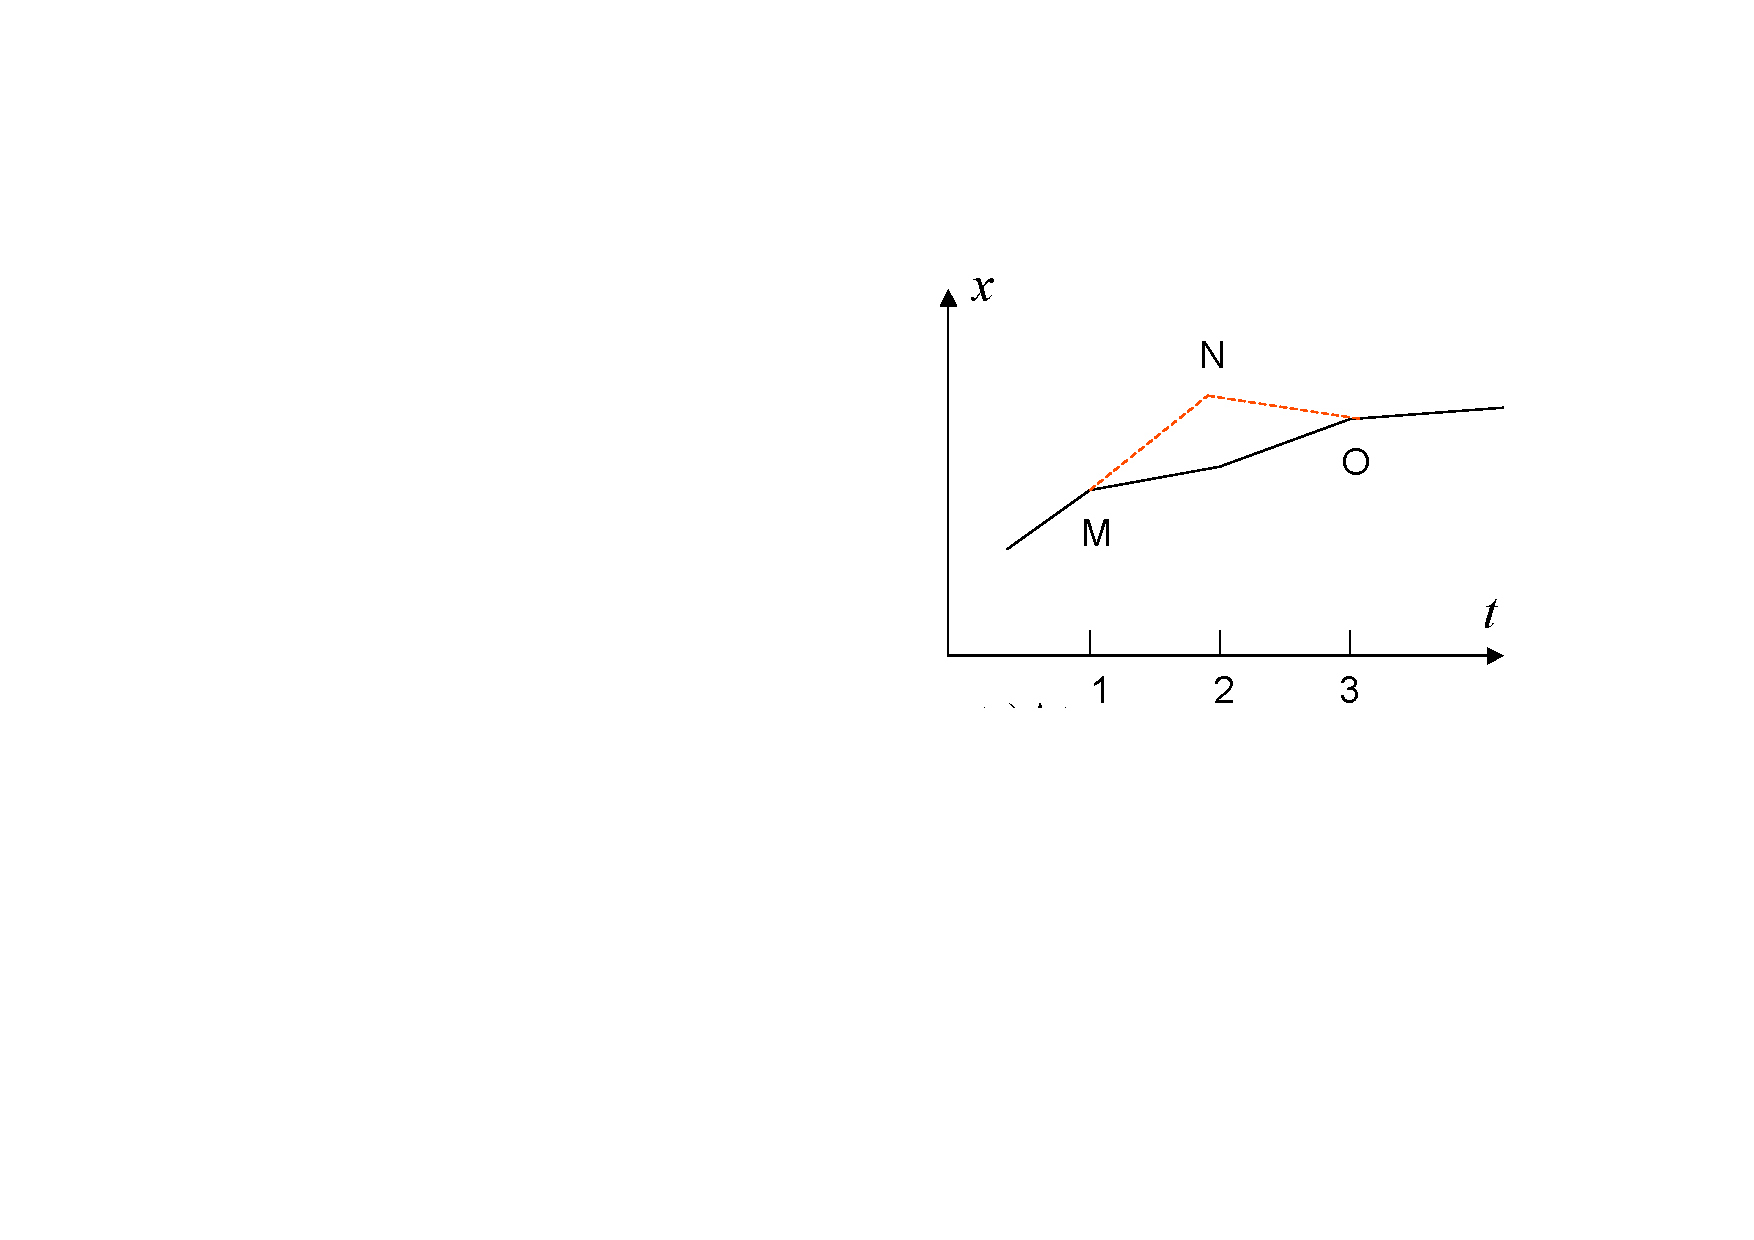
\includegraphics[width=0.5\textwidth]{./graphs/action-path.pdf}
\end{figure}
%%%
%

% position of a point
\newcommand{\pospoint}[1]{\comp{\pvec}{\point{#1}}}
% average velocity of a point
\newcommand{\avelpoint}[1]{\comp{\bar{\pvec}}{\point{#1}}}

The key observation, due to Euler, is that every section of the action integral, or sum in this case, must be stationary; \ie, it must take either a maximum or a minimum value. To see this, refer to \cref{fig:approxpath}. To find this stationary value, refer again to the figure. It shows a linearized path with the points $\point M$ and $\point O$ on it. The point between them, $\point N$ at time $t_2$, was shifted from the linearized path (approximation of the real path taken by a particle) to a higher position. Note in the figure that the positions of $\point M$, $\pospoint M$, and of $\point O$, $\pospoint O$, are fixed. 

Next, calculate the value of the action between the three points, $\action_{\point M\point N\point O}$, as the sum of the actions of the component line segments, remembering that each $\comp xi$ is taken at the beginning of each segment
\beq
\action_{\point M\point N\point O} = \lag\vat{\pospoint M, \avelpoint M, t_1}\diff t 
                                   + \lag\vat{\pospoint N, \avelpoint N, t_2}\diff t\,.
\eeq

Without loss of generality, take equal time steps: $\diff t = t_2 - t_1 = t_3 - t_2$. Then, $\avelpoint M = (\pospoint N - \pospoint M)/\diff t$ and $\avelpoint N = (\pospoint O - \pospoint N)/\diff t$.

Require then the action to be stationary noting that $\action$ is a function of $\pospoint N$ only, since the positions $\pospoint M$ and $\pospoint O$ are fixed, and using the chain rule for derivatives:
\beq
\xod{\action_{\point M\point N\point O}}{\pospoint N} 
    = \left( 
      \xpd{\lag}{\avelpoint M}\xod{\avelpoint M}{\pospoint N} 
      + \xpd{\lag}{\pospoint N}
      + \xpd{\lag}{\avelpoint N}\xod{\avelpoint N}{\pospoint N} 
      \right) \diff t = 0\,.
\eeq

Note that $\dx\avelpoint M/\dx\pospoint N = 1/\diff t$ and $\dx\avelpoint N/\dx\pospoint N = -1/\diff t$ to have
\beq
\xod{\action_{\point M\point N\point O}}{\pospoint N} 
    = \left( 
      \xpd{\lag}{\avelpoint M}\dfrac{1}{\diff t}
      + \xpd{\lag}{\pospoint N}
      - \xpd{\lag}{\avelpoint N}\dfrac{1}{\diff t} 
      \right) \diff t 
    = \xpd{\lag}{\pospoint N}
      - \dfrac{1}{\diff t}
      \left( 
      \xpd{\lag}{\avelpoint N}
      -\xpd{\lag}{\avelpoint M}
      \right)
    = 0\,.
\eeq

This last condition must hold for any point on the path, so taking $\diff t\to 0$, one has
\begin{equation}\label{eq:eleqngeometry}
\eleqn x{} = 0\,.
\end{equation}
This is to say that the condition that the action be stationary for every point of a particle trajectory implies that the particle's position $\pvec$ and velocity $\dt\pvec$ must satisfy \cref{eq:eleqngeometry}. This equation is called the Euler-Lagrange equation of motion and is the backbone of the Lagrangian description of motion, as opposed to the Newtonian description of motion.


\subsection{Classical test particle with Newtonian gravity}
Suppose we are given a particle with mass $m$ and position $\pvec\vat t$ in a Newtonian gravitation field with potential $\zeta$, where $\dim\zeta = \phdim{FL/M} = \phdim{E/M}$. The particle's world line is parameterized by time $t$. The particle's kinetic energy is~\footnote{~In geometric algebra, if $x$ is a vector, then $x^2 = xx = x\iprod x$, since $x$ is parallel to itself, and thus $x\oprod x = 0$.}
\beq
\ken\vat t = \dfrac{1}{2}m\dt\pvec^2\vat t
\eeq
and the particle's gravitational potential energy is
\beq
\pen\vat t = m\zeta\vat{\pvec\vat t, t}\,.
\eeq

Then the particle's Lagrangian is
\beq
\lag\vat t = \ken\vat t - \pen\vat t
           = \dfrac{1}{2}m\dt\pvec^2\vat t - m\zeta\vat{\pvec\vat t, t}\,.
\eeq

Varying $\pvec$ in the integral (equivalent to the Euler-Lagrange differential equation), we get
\beq
0 = \delta\int\lag\vat t\,\dx t 
  = \int\delta\lag\vat t\,\dx t
  = \int\left( m\dt\pvec\vat t\iprod \delta\dt\pvec\vat t
               - m\zeta\vat{\pvec\vat t, t}\iprod\delta\pvec\vat t
         \right)\,\dx t\,.
\eeq

Integrate the first term by parts and discard the total integral. Then divide out the variation to get
\beq
0 = -m\ddt\pvec\vat t - m\gder\zeta\vat{\pvec\vat t, t}
\eeq
and thus
\beq
m\ddt\pvec\vat t = - m\gder\zeta\vat{\pvec\vat t, t}
\eeq
is the equation of motion -- two different expressions for the force.


\subsection{Lagrangian in Vector Notation}
Using Lagrange's mechanics and vector calculus, find the equations of motion for a free particle of mass $m$.

\begin{solution}
The particle kinetic energy is $2\ken\vattpvec = m\dt\pvec^2\vat t$. Then, the particle Lagrangian becomes
\beq
\lag\vattpvec = \dfrac{1}{2}m\dt\pvec^2\vat t\,.
\eeq

Using the particle Langrangian, find the generalized force, generalized momentum and the generalized momentum time derivative
\beq
\xpd{\lag}{\pvec} = 0\,,\qquad
\xpd{\lag}{\dt\pvec} = m\dt\pvec\vat t\qquad\text{and}\qquad
\xod{}{t}\xpd{\lag}{\dt\pvec} = m\ddt\pvec\vat t\,.
\eeq

Euler-Lagrange's equations give finally the particle equations of motion:
\beq
\eleqn{\pvec}{} = m\ddt\pvec\vat t = 0\implies 
\ddt\pvec\vat t = 0\,.\mqed
\eeq
\end{solution}


Consider the last exercise particle to be object of a potential $\pen\vattpvec$. Find the particle equations of motion.

\begin{solution}
The particle Lagrangian becomes
\beq
\lag\vattpvec = \dfrac{1}{2}m\dt\pvec^2\vat t - \pen\vattpvec\,.
\eeq

Then, the generalized force, momentum and its time derivative are
\beq
\xpd{\lag}{\pvec} = -\xpd{\pen\vattpvec}{\pvec} = -\gder\pen\vattpvec \,,\qquad
\xpd{\lag}{\dt\pvec} = m\dt\pvec\vat t\qquad\text{and}\qquad
\xod{}{t}\xpd{\lag}{\dt\pvec} = m\ddt\pvec\vat t\,.
\eeq

Euler-Lagrange's equations give finally the particle equations of motion:
\beq
\eleqn{\pvec}{} = m\ddt\pvec\vat t + \gder\pen\vattpvec = 0\implies 
\ddt\pvec\vat t = -\gder\pen\vattpvec \,.\mqed
\eeq
\end{solution}



